\documentclass[
		book,
		head_space=20mm,
		foot_space=20mm,
		gutter=10mm,
		line_length=190mm
]{jlreq}

%----------
%LuaLaTeXで実行する!!
%----------
%各章節には以下を書く. 1-03.texのような名前にする
%----------
% \documentclass[
% 		book,
% 		head_space=20mm,
% 		foot_space=20mm,
% 		gutter=10mm,
% 		line_length=190mm
% ]{jlreq}
% 
%----------
%LuaLaTeXで実行する!!
%----------
%各章節には以下を書く. 1-03.texのような名前にする
%----------
% \documentclass[
% 		book,
% 		head_space=20mm,
% 		foot_space=20mm,
% 		gutter=10mm,
% 		line_length=190mm
% ]{jlreq}
% 
%----------
%LuaLaTeXで実行する!!
%----------
%各章節には以下を書く. 1-03.texのような名前にする
%----------
% \documentclass[
% 		book,
% 		head_space=20mm,
% 		foot_space=20mm,
% 		gutter=10mm,
% 		line_length=190mm
% ]{jlreq}
% \input {preamble.tex}
% \usepackage{docmute} %ファイル分割
% \begin{document}

% %\chapter{章のタイトル}
% \section{節のタイトル}
% no text

% \end{document}
%----------

%main.texには以下を書く
%----------
% \documentclass[
% 		book,
% 		head_space=20mm,
% 		foot_space=20mm,
% 		gutter=10mm,
% 		line_length=190mm,
%         openany
% ]{jlreq}
% \input {preamble.tex}
% \usepackage{docmute} %ファイル分割
% \begin{document}

% %---------- 1章1節
% \input 1-01.tex
% %---------- 1章2節
% \input 1-02.tex
% % ---------- 1章3節
% \input 1-03.tex
% % ---------- 1章4節
% \input 1-04.tex
% % ---------- 1章5節
% \input 1-05.tex
% % ---------- 1章6節
% \input 1-06.tex
% %---------- 1章7節
% \input 1-07.tex
% % ---------- 1章8節
% \input 1-08.tex
% % ---------- 1章9節
% \input 1-09.tex
% % ---------- 1章10節
% \input 1-10.tex
% % ---------- 1章11節
% \input 1-11.tex
% % ---------- 1章12節
% \input 1-12.tex
% % ---------- 参考文献
% \input reference.tex
% \end{document}
% ----------



\usepackage{bxtexlogo}
\usepackage{amsthm}
\usepackage{amsmath}
\usepackage{bbm} %小文字の黒板文字
\usepackage{physics}
\usepackage{amsfonts}
\usepackage{graphicx}
\usepackage{mathtools}
\usepackage{enumitem}
\usepackage[margin=20truemm]{geometry}
\usepackage{textcomp}
\usepackage{bm}
\usepackage{mathrsfs}
\usepackage{latexsym}
\usepackage{amssymb}
\usepackage{algorithmic}
\usepackage{algorithm}
\usepackage{tikz}
\usetikzlibrary{arrows.meta}
\usetikzlibrary{math,matrix,backgrounds}
\usetikzlibrary{angles}
\usetikzlibrary{calc}


%----------
%日本語フォント
% \usepackage[deluxe]{otf} platex用 lualatexでは動かない

%----------
%欧文フォント
\usepackage[T1]{fontenc}

%----------
%文字色
\usepackage{color}

%----------
\setlength{\parindent}{2\zw} %インデントの設定

%----------
% %参照した数式にだけ番号を振る cleverrefと併用するとうまくいかない
% \mathtoolsset{showonlyrefs=true}
%----------

%----------
%集合の中線
\newcommand{\relmiddle}[1]{\mathrel{}\middle#1\mathrel{}}
% \middle| の代わりに \relmiddle| を付ける
\newcommand{\sgn}{\mathop{\mathrm{sgn}}} %置換sgn
\newcommand{\Int}{\mathop{\mathrm{Int}}} %位相空間の内部Int
\newcommand{\Ext}{\mathop{\mathrm{Ext}}} %位相空間の外部Ext
\newcommand{\Cl}{\mathop{\mathrm{Cl}}} %位相空間の閉包Cl
\newcommand{\supp}{\mathop{\mathrm{supp}}} %関数の台supp
\newcommand{\restrict}[2]{\left. #1 \right \vert_{#2}}%関数の制限 \restrict{f}{A} = f|_A
\newcommand{\Ker}{\mathop{\mathrm{Ker}}}
\newcommand{\Coker}{\mathop{\mathrm{Coker}}}
\newcommand{\coker}{\mathop{\mathrm{coker}}}
\newcommand{\Coim}{\mathop{\mathrm{Coim}}}
\newcommand{\coim}{\mathop{\mathrm{coim}}}
\newcommand{\id}{\mathop{\mathrm{id}}}
\newcommand{\Gal}{\mathop{\mathrm{Gal}}}

\newtheorem{definition}{定義}[section]

\usepackage{aliascnt}

% \newaliastheorem{(環境とカウンターの名前)}{(元となるカウンターの名前)}{(表示される文字列)}
\newcommand*{\newaliastheorem}[3]{%
  \newaliascnt{#1}{#2}%
  \newtheorem{#1}[#1]{#3}%
  \aliascntresetthe{#1}%
  \expandafter\newcommand\csname #1autorefname\endcsname{#3}%
}
\newaliastheorem{proposition}{definition}{命題} 
\newaliastheorem{theorem}{definition}{定理}
\newaliastheorem{lemma}{definition}{補題}
\newaliastheorem{corollary}{definition}{系}
\newaliastheorem{example}{definition}{例}
\newaliastheorem{practice}{definition}{演習問題}

\newtheorem*{longproof}{証明}
\newtheorem*{answer}{解答}
\newtheorem*{supplement}{補足}
\newtheorem*{remark}{注意}
%----------

%----------
%古い記法を注意するパッケージ
\RequirePackage[l2tabu, orthodox]{nag}
%----------


% 定理環境(tcolorbox)
\usepackage{tcolorbox} %箱
\tcbuselibrary{breakable,skins,theorems}
\tcolorboxenvironment{definition}{
	blanker,breakable,
	left=3mm,right=3mm,
	top=2mm,bottom=2mm,
	before skip=15pt,after skip=20pt,
	borderline ={0.5pt}{0pt}{black}
}
\newtcolorbox{emptydefinition}{
	blanker,breakable,
	left=3mm,right=3mm,
	top=2mm,bottom=2mm,
	before skip=15pt,after skip=20pt,
	borderline ={0.5pt}{0pt}{black}
}
%----------
\tcolorboxenvironment{proposition}{
	blanker,breakable,
	left=3mm,right=3mm,
	top=3mm,bottom=3mm,
	before skip=15pt,after skip=15pt,
	borderline={0.5pt}{0pt}{black}
}
\newtcolorbox{emptyproposition}{
	blanker,breakable,
	left=3mm,right=3mm,
	top=3mm,bottom=3mm,
	before skip=15pt,after skip=15pt,
	borderline={0.5pt}{0pt}{black}
}
%----------
\tcolorboxenvironment{theorem}{
	blanker,breakable,
	left=3mm,right=3mm,
	top=3mm,bottom=3mm,
    sharp corners,boxrule=0.6pt,
	before skip=15pt,after skip=15pt,
	borderline={0.5pt}{0pt}{black},
    borderline={0.5pt}{1.5pt}{black}
}
\newtcolorbox{emptytheorem}{
	blanker,breakable,
	left=3mm,right=3mm,
	top=3mm,bottom=3mm,
    sharp corners,boxrule=0.6pt,
	before skip=15pt,after skip=15pt,
	borderline={0.5pt}{0pt}{black},
    borderline={0.5pt}{1.5pt}{black}
}
%----------
\tcolorboxenvironment{lemma}{
	blanker,breakable,
	left=3mm,right=3mm,
	top=3mm,bottom=3mm,
	before skip=15pt,after skip=15pt,
	borderline={0.5pt}{0pt}{black}
}
%----------
\tcolorboxenvironment{corollary}{
	blanker,breakable,
	left=3mm,right=3mm,
	top=3mm,bottom=3mm,
	before skip=15pt,after skip=15pt,
	borderline={1.0pt}{0pt}{black,dotted}
}
\newtcolorbox{emptycorollary}{
	blanker,breakable,
	left=3mm,right=3mm,
	top=3mm,bottom=3mm,
	before skip=15pt,after skip=15pt,
	borderline={1.0pt}{0pt}{black,dotted}
}
%----------
\tcolorboxenvironment{example}{
	blanker,breakable,
	left=3mm,right=3mm,
	top=3mm,bottom=3mm,
	before skip=15pt,after skip=15pt,
	borderline={0.5pt}{0pt}{black}
}
%----------
\tcolorboxenvironment{practice}{
	blanker,breakable,
	left=3mm,right=3mm,
	top=3mm,bottom=3mm,
	before skip=15pt,after skip=15pt,
	borderline={0.5pt}{0pt}{black}
}
%----------
\tcolorboxenvironment{proof}{
	blanker,breakable,
	left=3mm,right=3mm,
	top=2mm,bottom=2mm,
	before skip=15pt,after skip=20pt,
	% borderline west={1.5pt}{0pt}{black,dotted}
	borderline vertical={1pt}{0pt}{black,dotted}
	% borderline vertical={0.8pt}{0pt}{black,dotted,arrows={Square[scale=0.5]-Square[scale=0.5]}}
	}
%----------
\tcolorboxenvironment{supplement}{
	blanker,breakable,
	left=3mm,right=3mm,
	top=2mm,bottom=2mm,
	before skip=15pt,after skip=20pt,
	% borderline west={1.5pt}{0pt}{black,dotted}
	% borderline vertical={0.5pt}{0pt}{black,arrows = {Circle[scale=0.7]-Circle[scale=0.7]}}
	borderline vertical={0.5pt}{0pt}{black}
	% borderline vertical={0.5pt}{0pt}{black},
	% borderline north={0.5pt}{0pt}{white,arrows={Circle[black,scale=0.7]-Circle[black,scale=0.7]}}
	}
%----------
\tcolorboxenvironment{remark}{
	blanker,breakable,
	left=3mm,right=3mm,
	top=1mm,bottom=1mm,
	before skip=15pt,after skip=20pt,
	% borderline west={1.5pt}{0pt}{black,dotted}
	% borderline vertical={0.5pt}{0pt}{black,arrows = {Circle[scale=0.7]-Circle[scale=0.7]}}
	borderline vertical={0.5pt}{0pt}{black}
	% borderline vertical={0.5pt}{0pt}{black},
	% borderline north={0.5pt}{0pt}{white,arrows={Circle[black,scale=0.7]-Circle[black,scale=0.7]}}
	}
    
%---------------------
 

%----------
%ハイパーリンク
% 「%」は以降の内容を「改行コードも含めて」無視するコマンド
\usepackage[%
%  dvipdfmx,% 欧文ではコメントアウトする
luatex,%
pdfencoding=auto,%
 setpagesize=false,%
 bookmarks=true,%
 bookmarksdepth=tocdepth,%
 bookmarksnumbered=true,%
 colorlinks=false,%
 pdftitle={},%
 pdfsubject={},%
 pdfauthor={},%
 pdfkeywords={}%
]{hyperref}
%------------


%参照 参照するときに自動で環境名を含んで参照する
\usepackage[nameinlink]{cleveref}
\let\normalref\ref
\renewcommand{\ref}{\cref}
\crefname{definition}{定義}{定義}
\crefname{proposition}{命題}{命題}
\crefname{theorem}{定理}{定理}
\crefname{lemma}{補題}{補題}
\crefname{corollary}{系}{系}
\crefname{example}{例}{例}
\crefname{practice}{演習問題}{演習問題}
\crefname{equation}{式}{式} 
\crefname{chapter}{第}{第}
\creflabelformat{chapter}{#2#1章#3}
\crefname{section}{第}{第}
\creflabelformat{section}{#2#1節#3}
\crefname{subsection}{第}{第}
\creflabelformat{subsection}{#2#1小節#3}
%----------

%---------------------
%章跨ぎの参照が不具合を起こすための代わり
% \mylabl でラベル付け
\newcommand{\mylabel}[1]{
\label{#1}
\hypertarget{#1}{}
}
% \myref で環境名付きリンクをつける
\newcommand{\myref}[1]{
\hyperlink{#1}{\cref*{#1}}
}
%-----------------

\usepackage{autonum} %参照した数式にだけ番号を振る
% \usepackage{docmute} %ファイル分割
% \begin{document}

% %\chapter{章のタイトル}
% \section{節のタイトル}
% no text

% \end{document}
%----------

%main.texには以下を書く
%----------
% \documentclass[
% 		book,
% 		head_space=20mm,
% 		foot_space=20mm,
% 		gutter=10mm,
% 		line_length=190mm,
%         openany
% ]{jlreq}
% 
%----------
%LuaLaTeXで実行する!!
%----------
%各章節には以下を書く. 1-03.texのような名前にする
%----------
% \documentclass[
% 		book,
% 		head_space=20mm,
% 		foot_space=20mm,
% 		gutter=10mm,
% 		line_length=190mm
% ]{jlreq}
% \input {preamble.tex}
% \usepackage{docmute} %ファイル分割
% \begin{document}

% %\chapter{章のタイトル}
% \section{節のタイトル}
% no text

% \end{document}
%----------

%main.texには以下を書く
%----------
% \documentclass[
% 		book,
% 		head_space=20mm,
% 		foot_space=20mm,
% 		gutter=10mm,
% 		line_length=190mm,
%         openany
% ]{jlreq}
% \input {preamble.tex}
% \usepackage{docmute} %ファイル分割
% \begin{document}

% %---------- 1章1節
% \input 1-01.tex
% %---------- 1章2節
% \input 1-02.tex
% % ---------- 1章3節
% \input 1-03.tex
% % ---------- 1章4節
% \input 1-04.tex
% % ---------- 1章5節
% \input 1-05.tex
% % ---------- 1章6節
% \input 1-06.tex
% %---------- 1章7節
% \input 1-07.tex
% % ---------- 1章8節
% \input 1-08.tex
% % ---------- 1章9節
% \input 1-09.tex
% % ---------- 1章10節
% \input 1-10.tex
% % ---------- 1章11節
% \input 1-11.tex
% % ---------- 1章12節
% \input 1-12.tex
% % ---------- 参考文献
% \input reference.tex
% \end{document}
% ----------



\usepackage{bxtexlogo}
\usepackage{amsthm}
\usepackage{amsmath}
\usepackage{bbm} %小文字の黒板文字
\usepackage{physics}
\usepackage{amsfonts}
\usepackage{graphicx}
\usepackage{mathtools}
\usepackage{enumitem}
\usepackage[margin=20truemm]{geometry}
\usepackage{textcomp}
\usepackage{bm}
\usepackage{mathrsfs}
\usepackage{latexsym}
\usepackage{amssymb}
\usepackage{algorithmic}
\usepackage{algorithm}
\usepackage{tikz}
\usetikzlibrary{arrows.meta}
\usetikzlibrary{math,matrix,backgrounds}
\usetikzlibrary{angles}
\usetikzlibrary{calc}


%----------
%日本語フォント
% \usepackage[deluxe]{otf} platex用 lualatexでは動かない

%----------
%欧文フォント
\usepackage[T1]{fontenc}

%----------
%文字色
\usepackage{color}

%----------
\setlength{\parindent}{2\zw} %インデントの設定

%----------
% %参照した数式にだけ番号を振る cleverrefと併用するとうまくいかない
% \mathtoolsset{showonlyrefs=true}
%----------

%----------
%集合の中線
\newcommand{\relmiddle}[1]{\mathrel{}\middle#1\mathrel{}}
% \middle| の代わりに \relmiddle| を付ける
\newcommand{\sgn}{\mathop{\mathrm{sgn}}} %置換sgn
\newcommand{\Int}{\mathop{\mathrm{Int}}} %位相空間の内部Int
\newcommand{\Ext}{\mathop{\mathrm{Ext}}} %位相空間の外部Ext
\newcommand{\Cl}{\mathop{\mathrm{Cl}}} %位相空間の閉包Cl
\newcommand{\supp}{\mathop{\mathrm{supp}}} %関数の台supp
\newcommand{\restrict}[2]{\left. #1 \right \vert_{#2}}%関数の制限 \restrict{f}{A} = f|_A
\newcommand{\Ker}{\mathop{\mathrm{Ker}}}
\newcommand{\Coker}{\mathop{\mathrm{Coker}}}
\newcommand{\coker}{\mathop{\mathrm{coker}}}
\newcommand{\Coim}{\mathop{\mathrm{Coim}}}
\newcommand{\coim}{\mathop{\mathrm{coim}}}
\newcommand{\id}{\mathop{\mathrm{id}}}
\newcommand{\Gal}{\mathop{\mathrm{Gal}}}

\newtheorem{definition}{定義}[section]

\usepackage{aliascnt}

% \newaliastheorem{(環境とカウンターの名前)}{(元となるカウンターの名前)}{(表示される文字列)}
\newcommand*{\newaliastheorem}[3]{%
  \newaliascnt{#1}{#2}%
  \newtheorem{#1}[#1]{#3}%
  \aliascntresetthe{#1}%
  \expandafter\newcommand\csname #1autorefname\endcsname{#3}%
}
\newaliastheorem{proposition}{definition}{命題} 
\newaliastheorem{theorem}{definition}{定理}
\newaliastheorem{lemma}{definition}{補題}
\newaliastheorem{corollary}{definition}{系}
\newaliastheorem{example}{definition}{例}
\newaliastheorem{practice}{definition}{演習問題}

\newtheorem*{longproof}{証明}
\newtheorem*{answer}{解答}
\newtheorem*{supplement}{補足}
\newtheorem*{remark}{注意}
%----------

%----------
%古い記法を注意するパッケージ
\RequirePackage[l2tabu, orthodox]{nag}
%----------


% 定理環境(tcolorbox)
\usepackage{tcolorbox} %箱
\tcbuselibrary{breakable,skins,theorems}
\tcolorboxenvironment{definition}{
	blanker,breakable,
	left=3mm,right=3mm,
	top=2mm,bottom=2mm,
	before skip=15pt,after skip=20pt,
	borderline ={0.5pt}{0pt}{black}
}
\newtcolorbox{emptydefinition}{
	blanker,breakable,
	left=3mm,right=3mm,
	top=2mm,bottom=2mm,
	before skip=15pt,after skip=20pt,
	borderline ={0.5pt}{0pt}{black}
}
%----------
\tcolorboxenvironment{proposition}{
	blanker,breakable,
	left=3mm,right=3mm,
	top=3mm,bottom=3mm,
	before skip=15pt,after skip=15pt,
	borderline={0.5pt}{0pt}{black}
}
\newtcolorbox{emptyproposition}{
	blanker,breakable,
	left=3mm,right=3mm,
	top=3mm,bottom=3mm,
	before skip=15pt,after skip=15pt,
	borderline={0.5pt}{0pt}{black}
}
%----------
\tcolorboxenvironment{theorem}{
	blanker,breakable,
	left=3mm,right=3mm,
	top=3mm,bottom=3mm,
    sharp corners,boxrule=0.6pt,
	before skip=15pt,after skip=15pt,
	borderline={0.5pt}{0pt}{black},
    borderline={0.5pt}{1.5pt}{black}
}
\newtcolorbox{emptytheorem}{
	blanker,breakable,
	left=3mm,right=3mm,
	top=3mm,bottom=3mm,
    sharp corners,boxrule=0.6pt,
	before skip=15pt,after skip=15pt,
	borderline={0.5pt}{0pt}{black},
    borderline={0.5pt}{1.5pt}{black}
}
%----------
\tcolorboxenvironment{lemma}{
	blanker,breakable,
	left=3mm,right=3mm,
	top=3mm,bottom=3mm,
	before skip=15pt,after skip=15pt,
	borderline={0.5pt}{0pt}{black}
}
%----------
\tcolorboxenvironment{corollary}{
	blanker,breakable,
	left=3mm,right=3mm,
	top=3mm,bottom=3mm,
	before skip=15pt,after skip=15pt,
	borderline={1.0pt}{0pt}{black,dotted}
}
\newtcolorbox{emptycorollary}{
	blanker,breakable,
	left=3mm,right=3mm,
	top=3mm,bottom=3mm,
	before skip=15pt,after skip=15pt,
	borderline={1.0pt}{0pt}{black,dotted}
}
%----------
\tcolorboxenvironment{example}{
	blanker,breakable,
	left=3mm,right=3mm,
	top=3mm,bottom=3mm,
	before skip=15pt,after skip=15pt,
	borderline={0.5pt}{0pt}{black}
}
%----------
\tcolorboxenvironment{practice}{
	blanker,breakable,
	left=3mm,right=3mm,
	top=3mm,bottom=3mm,
	before skip=15pt,after skip=15pt,
	borderline={0.5pt}{0pt}{black}
}
%----------
\tcolorboxenvironment{proof}{
	blanker,breakable,
	left=3mm,right=3mm,
	top=2mm,bottom=2mm,
	before skip=15pt,after skip=20pt,
	% borderline west={1.5pt}{0pt}{black,dotted}
	borderline vertical={1pt}{0pt}{black,dotted}
	% borderline vertical={0.8pt}{0pt}{black,dotted,arrows={Square[scale=0.5]-Square[scale=0.5]}}
	}
%----------
\tcolorboxenvironment{supplement}{
	blanker,breakable,
	left=3mm,right=3mm,
	top=2mm,bottom=2mm,
	before skip=15pt,after skip=20pt,
	% borderline west={1.5pt}{0pt}{black,dotted}
	% borderline vertical={0.5pt}{0pt}{black,arrows = {Circle[scale=0.7]-Circle[scale=0.7]}}
	borderline vertical={0.5pt}{0pt}{black}
	% borderline vertical={0.5pt}{0pt}{black},
	% borderline north={0.5pt}{0pt}{white,arrows={Circle[black,scale=0.7]-Circle[black,scale=0.7]}}
	}
%----------
\tcolorboxenvironment{remark}{
	blanker,breakable,
	left=3mm,right=3mm,
	top=1mm,bottom=1mm,
	before skip=15pt,after skip=20pt,
	% borderline west={1.5pt}{0pt}{black,dotted}
	% borderline vertical={0.5pt}{0pt}{black,arrows = {Circle[scale=0.7]-Circle[scale=0.7]}}
	borderline vertical={0.5pt}{0pt}{black}
	% borderline vertical={0.5pt}{0pt}{black},
	% borderline north={0.5pt}{0pt}{white,arrows={Circle[black,scale=0.7]-Circle[black,scale=0.7]}}
	}
    
%---------------------
 

%----------
%ハイパーリンク
% 「%」は以降の内容を「改行コードも含めて」無視するコマンド
\usepackage[%
%  dvipdfmx,% 欧文ではコメントアウトする
luatex,%
pdfencoding=auto,%
 setpagesize=false,%
 bookmarks=true,%
 bookmarksdepth=tocdepth,%
 bookmarksnumbered=true,%
 colorlinks=false,%
 pdftitle={},%
 pdfsubject={},%
 pdfauthor={},%
 pdfkeywords={}%
]{hyperref}
%------------


%参照 参照するときに自動で環境名を含んで参照する
\usepackage[nameinlink]{cleveref}
\let\normalref\ref
\renewcommand{\ref}{\cref}
\crefname{definition}{定義}{定義}
\crefname{proposition}{命題}{命題}
\crefname{theorem}{定理}{定理}
\crefname{lemma}{補題}{補題}
\crefname{corollary}{系}{系}
\crefname{example}{例}{例}
\crefname{practice}{演習問題}{演習問題}
\crefname{equation}{式}{式} 
\crefname{chapter}{第}{第}
\creflabelformat{chapter}{#2#1章#3}
\crefname{section}{第}{第}
\creflabelformat{section}{#2#1節#3}
\crefname{subsection}{第}{第}
\creflabelformat{subsection}{#2#1小節#3}
%----------

%---------------------
%章跨ぎの参照が不具合を起こすための代わり
% \mylabl でラベル付け
\newcommand{\mylabel}[1]{
\label{#1}
\hypertarget{#1}{}
}
% \myref で環境名付きリンクをつける
\newcommand{\myref}[1]{
\hyperlink{#1}{\cref*{#1}}
}
%-----------------

\usepackage{autonum} %参照した数式にだけ番号を振る
% \usepackage{docmute} %ファイル分割
% \begin{document}

% %---------- 1章1節
% \input 1-01.tex
% %---------- 1章2節
% \input 1-02.tex
% % ---------- 1章3節
% \input 1-03.tex
% % ---------- 1章4節
% \input 1-04.tex
% % ---------- 1章5節
% \input 1-05.tex
% % ---------- 1章6節
% \input 1-06.tex
% %---------- 1章7節
% \input 1-07.tex
% % ---------- 1章8節
% \input 1-08.tex
% % ---------- 1章9節
% \input 1-09.tex
% % ---------- 1章10節
% \input 1-10.tex
% % ---------- 1章11節
% \input 1-11.tex
% % ---------- 1章12節
% \input 1-12.tex
% % ---------- 参考文献
% \input reference.tex
% \end{document}
% ----------



\usepackage{bxtexlogo}
\usepackage{amsthm}
\usepackage{amsmath}
\usepackage{bbm} %小文字の黒板文字
\usepackage{physics}
\usepackage{amsfonts}
\usepackage{graphicx}
\usepackage{mathtools}
\usepackage{enumitem}
\usepackage[margin=20truemm]{geometry}
\usepackage{textcomp}
\usepackage{bm}
\usepackage{mathrsfs}
\usepackage{latexsym}
\usepackage{amssymb}
\usepackage{algorithmic}
\usepackage{algorithm}
\usepackage{tikz}
\usetikzlibrary{arrows.meta}
\usetikzlibrary{math,matrix,backgrounds}
\usetikzlibrary{angles}
\usetikzlibrary{calc}


%----------
%日本語フォント
% \usepackage[deluxe]{otf} platex用 lualatexでは動かない

%----------
%欧文フォント
\usepackage[T1]{fontenc}

%----------
%文字色
\usepackage{color}

%----------
\setlength{\parindent}{2\zw} %インデントの設定

%----------
% %参照した数式にだけ番号を振る cleverrefと併用するとうまくいかない
% \mathtoolsset{showonlyrefs=true}
%----------

%----------
%集合の中線
\newcommand{\relmiddle}[1]{\mathrel{}\middle#1\mathrel{}}
% \middle| の代わりに \relmiddle| を付ける
\newcommand{\sgn}{\mathop{\mathrm{sgn}}} %置換sgn
\newcommand{\Int}{\mathop{\mathrm{Int}}} %位相空間の内部Int
\newcommand{\Ext}{\mathop{\mathrm{Ext}}} %位相空間の外部Ext
\newcommand{\Cl}{\mathop{\mathrm{Cl}}} %位相空間の閉包Cl
\newcommand{\supp}{\mathop{\mathrm{supp}}} %関数の台supp
\newcommand{\restrict}[2]{\left. #1 \right \vert_{#2}}%関数の制限 \restrict{f}{A} = f|_A
\newcommand{\Ker}{\mathop{\mathrm{Ker}}}
\newcommand{\Coker}{\mathop{\mathrm{Coker}}}
\newcommand{\coker}{\mathop{\mathrm{coker}}}
\newcommand{\Coim}{\mathop{\mathrm{Coim}}}
\newcommand{\coim}{\mathop{\mathrm{coim}}}
\newcommand{\id}{\mathop{\mathrm{id}}}
\newcommand{\Gal}{\mathop{\mathrm{Gal}}}

\newtheorem{definition}{定義}[section]

\usepackage{aliascnt}

% \newaliastheorem{(環境とカウンターの名前)}{(元となるカウンターの名前)}{(表示される文字列)}
\newcommand*{\newaliastheorem}[3]{%
  \newaliascnt{#1}{#2}%
  \newtheorem{#1}[#1]{#3}%
  \aliascntresetthe{#1}%
  \expandafter\newcommand\csname #1autorefname\endcsname{#3}%
}
\newaliastheorem{proposition}{definition}{命題} 
\newaliastheorem{theorem}{definition}{定理}
\newaliastheorem{lemma}{definition}{補題}
\newaliastheorem{corollary}{definition}{系}
\newaliastheorem{example}{definition}{例}
\newaliastheorem{practice}{definition}{演習問題}

\newtheorem*{longproof}{証明}
\newtheorem*{answer}{解答}
\newtheorem*{supplement}{補足}
\newtheorem*{remark}{注意}
%----------

%----------
%古い記法を注意するパッケージ
\RequirePackage[l2tabu, orthodox]{nag}
%----------


% 定理環境(tcolorbox)
\usepackage{tcolorbox} %箱
\tcbuselibrary{breakable,skins,theorems}
\tcolorboxenvironment{definition}{
	blanker,breakable,
	left=3mm,right=3mm,
	top=2mm,bottom=2mm,
	before skip=15pt,after skip=20pt,
	borderline ={0.5pt}{0pt}{black}
}
\newtcolorbox{emptydefinition}{
	blanker,breakable,
	left=3mm,right=3mm,
	top=2mm,bottom=2mm,
	before skip=15pt,after skip=20pt,
	borderline ={0.5pt}{0pt}{black}
}
%----------
\tcolorboxenvironment{proposition}{
	blanker,breakable,
	left=3mm,right=3mm,
	top=3mm,bottom=3mm,
	before skip=15pt,after skip=15pt,
	borderline={0.5pt}{0pt}{black}
}
\newtcolorbox{emptyproposition}{
	blanker,breakable,
	left=3mm,right=3mm,
	top=3mm,bottom=3mm,
	before skip=15pt,after skip=15pt,
	borderline={0.5pt}{0pt}{black}
}
%----------
\tcolorboxenvironment{theorem}{
	blanker,breakable,
	left=3mm,right=3mm,
	top=3mm,bottom=3mm,
    sharp corners,boxrule=0.6pt,
	before skip=15pt,after skip=15pt,
	borderline={0.5pt}{0pt}{black},
    borderline={0.5pt}{1.5pt}{black}
}
\newtcolorbox{emptytheorem}{
	blanker,breakable,
	left=3mm,right=3mm,
	top=3mm,bottom=3mm,
    sharp corners,boxrule=0.6pt,
	before skip=15pt,after skip=15pt,
	borderline={0.5pt}{0pt}{black},
    borderline={0.5pt}{1.5pt}{black}
}
%----------
\tcolorboxenvironment{lemma}{
	blanker,breakable,
	left=3mm,right=3mm,
	top=3mm,bottom=3mm,
	before skip=15pt,after skip=15pt,
	borderline={0.5pt}{0pt}{black}
}
%----------
\tcolorboxenvironment{corollary}{
	blanker,breakable,
	left=3mm,right=3mm,
	top=3mm,bottom=3mm,
	before skip=15pt,after skip=15pt,
	borderline={1.0pt}{0pt}{black,dotted}
}
\newtcolorbox{emptycorollary}{
	blanker,breakable,
	left=3mm,right=3mm,
	top=3mm,bottom=3mm,
	before skip=15pt,after skip=15pt,
	borderline={1.0pt}{0pt}{black,dotted}
}
%----------
\tcolorboxenvironment{example}{
	blanker,breakable,
	left=3mm,right=3mm,
	top=3mm,bottom=3mm,
	before skip=15pt,after skip=15pt,
	borderline={0.5pt}{0pt}{black}
}
%----------
\tcolorboxenvironment{practice}{
	blanker,breakable,
	left=3mm,right=3mm,
	top=3mm,bottom=3mm,
	before skip=15pt,after skip=15pt,
	borderline={0.5pt}{0pt}{black}
}
%----------
\tcolorboxenvironment{proof}{
	blanker,breakable,
	left=3mm,right=3mm,
	top=2mm,bottom=2mm,
	before skip=15pt,after skip=20pt,
	% borderline west={1.5pt}{0pt}{black,dotted}
	borderline vertical={1pt}{0pt}{black,dotted}
	% borderline vertical={0.8pt}{0pt}{black,dotted,arrows={Square[scale=0.5]-Square[scale=0.5]}}
	}
%----------
\tcolorboxenvironment{supplement}{
	blanker,breakable,
	left=3mm,right=3mm,
	top=2mm,bottom=2mm,
	before skip=15pt,after skip=20pt,
	% borderline west={1.5pt}{0pt}{black,dotted}
	% borderline vertical={0.5pt}{0pt}{black,arrows = {Circle[scale=0.7]-Circle[scale=0.7]}}
	borderline vertical={0.5pt}{0pt}{black}
	% borderline vertical={0.5pt}{0pt}{black},
	% borderline north={0.5pt}{0pt}{white,arrows={Circle[black,scale=0.7]-Circle[black,scale=0.7]}}
	}
%----------
\tcolorboxenvironment{remark}{
	blanker,breakable,
	left=3mm,right=3mm,
	top=1mm,bottom=1mm,
	before skip=15pt,after skip=20pt,
	% borderline west={1.5pt}{0pt}{black,dotted}
	% borderline vertical={0.5pt}{0pt}{black,arrows = {Circle[scale=0.7]-Circle[scale=0.7]}}
	borderline vertical={0.5pt}{0pt}{black}
	% borderline vertical={0.5pt}{0pt}{black},
	% borderline north={0.5pt}{0pt}{white,arrows={Circle[black,scale=0.7]-Circle[black,scale=0.7]}}
	}
    
%---------------------
 

%----------
%ハイパーリンク
% 「%」は以降の内容を「改行コードも含めて」無視するコマンド
\usepackage[%
%  dvipdfmx,% 欧文ではコメントアウトする
luatex,%
pdfencoding=auto,%
 setpagesize=false,%
 bookmarks=true,%
 bookmarksdepth=tocdepth,%
 bookmarksnumbered=true,%
 colorlinks=false,%
 pdftitle={},%
 pdfsubject={},%
 pdfauthor={},%
 pdfkeywords={}%
]{hyperref}
%------------


%参照 参照するときに自動で環境名を含んで参照する
\usepackage[nameinlink]{cleveref}
\let\normalref\ref
\renewcommand{\ref}{\cref}
\crefname{definition}{定義}{定義}
\crefname{proposition}{命題}{命題}
\crefname{theorem}{定理}{定理}
\crefname{lemma}{補題}{補題}
\crefname{corollary}{系}{系}
\crefname{example}{例}{例}
\crefname{practice}{演習問題}{演習問題}
\crefname{equation}{式}{式} 
\crefname{chapter}{第}{第}
\creflabelformat{chapter}{#2#1章#3}
\crefname{section}{第}{第}
\creflabelformat{section}{#2#1節#3}
\crefname{subsection}{第}{第}
\creflabelformat{subsection}{#2#1小節#3}
%----------

%---------------------
%章跨ぎの参照が不具合を起こすための代わり
% \mylabl でラベル付け
\newcommand{\mylabel}[1]{
\label{#1}
\hypertarget{#1}{}
}
% \myref で環境名付きリンクをつける
\newcommand{\myref}[1]{
\hyperlink{#1}{\cref*{#1}}
}
%-----------------

\usepackage{autonum} %参照した数式にだけ番号を振る
% \usepackage{docmute} %ファイル分割
% \begin{document}

% %\chapter{章のタイトル}
% \section{節のタイトル}
% no text

% \end{document}
%----------

%main.texには以下を書く
%----------
% \documentclass[
% 		book,
% 		head_space=20mm,
% 		foot_space=20mm,
% 		gutter=10mm,
% 		line_length=190mm,
%         openany
% ]{jlreq}
% 
%----------
%LuaLaTeXで実行する!!
%----------
%各章節には以下を書く. 1-03.texのような名前にする
%----------
% \documentclass[
% 		book,
% 		head_space=20mm,
% 		foot_space=20mm,
% 		gutter=10mm,
% 		line_length=190mm
% ]{jlreq}
% 
%----------
%LuaLaTeXで実行する!!
%----------
%各章節には以下を書く. 1-03.texのような名前にする
%----------
% \documentclass[
% 		book,
% 		head_space=20mm,
% 		foot_space=20mm,
% 		gutter=10mm,
% 		line_length=190mm
% ]{jlreq}
% \input {preamble.tex}
% \usepackage{docmute} %ファイル分割
% \begin{document}

% %\chapter{章のタイトル}
% \section{節のタイトル}
% no text

% \end{document}
%----------

%main.texには以下を書く
%----------
% \documentclass[
% 		book,
% 		head_space=20mm,
% 		foot_space=20mm,
% 		gutter=10mm,
% 		line_length=190mm,
%         openany
% ]{jlreq}
% \input {preamble.tex}
% \usepackage{docmute} %ファイル分割
% \begin{document}

% %---------- 1章1節
% \input 1-01.tex
% %---------- 1章2節
% \input 1-02.tex
% % ---------- 1章3節
% \input 1-03.tex
% % ---------- 1章4節
% \input 1-04.tex
% % ---------- 1章5節
% \input 1-05.tex
% % ---------- 1章6節
% \input 1-06.tex
% %---------- 1章7節
% \input 1-07.tex
% % ---------- 1章8節
% \input 1-08.tex
% % ---------- 1章9節
% \input 1-09.tex
% % ---------- 1章10節
% \input 1-10.tex
% % ---------- 1章11節
% \input 1-11.tex
% % ---------- 1章12節
% \input 1-12.tex
% % ---------- 参考文献
% \input reference.tex
% \end{document}
% ----------



\usepackage{bxtexlogo}
\usepackage{amsthm}
\usepackage{amsmath}
\usepackage{bbm} %小文字の黒板文字
\usepackage{physics}
\usepackage{amsfonts}
\usepackage{graphicx}
\usepackage{mathtools}
\usepackage{enumitem}
\usepackage[margin=20truemm]{geometry}
\usepackage{textcomp}
\usepackage{bm}
\usepackage{mathrsfs}
\usepackage{latexsym}
\usepackage{amssymb}
\usepackage{algorithmic}
\usepackage{algorithm}
\usepackage{tikz}
\usetikzlibrary{arrows.meta}
\usetikzlibrary{math,matrix,backgrounds}
\usetikzlibrary{angles}
\usetikzlibrary{calc}


%----------
%日本語フォント
% \usepackage[deluxe]{otf} platex用 lualatexでは動かない

%----------
%欧文フォント
\usepackage[T1]{fontenc}

%----------
%文字色
\usepackage{color}

%----------
\setlength{\parindent}{2\zw} %インデントの設定

%----------
% %参照した数式にだけ番号を振る cleverrefと併用するとうまくいかない
% \mathtoolsset{showonlyrefs=true}
%----------

%----------
%集合の中線
\newcommand{\relmiddle}[1]{\mathrel{}\middle#1\mathrel{}}
% \middle| の代わりに \relmiddle| を付ける
\newcommand{\sgn}{\mathop{\mathrm{sgn}}} %置換sgn
\newcommand{\Int}{\mathop{\mathrm{Int}}} %位相空間の内部Int
\newcommand{\Ext}{\mathop{\mathrm{Ext}}} %位相空間の外部Ext
\newcommand{\Cl}{\mathop{\mathrm{Cl}}} %位相空間の閉包Cl
\newcommand{\supp}{\mathop{\mathrm{supp}}} %関数の台supp
\newcommand{\restrict}[2]{\left. #1 \right \vert_{#2}}%関数の制限 \restrict{f}{A} = f|_A
\newcommand{\Ker}{\mathop{\mathrm{Ker}}}
\newcommand{\Coker}{\mathop{\mathrm{Coker}}}
\newcommand{\coker}{\mathop{\mathrm{coker}}}
\newcommand{\Coim}{\mathop{\mathrm{Coim}}}
\newcommand{\coim}{\mathop{\mathrm{coim}}}
\newcommand{\id}{\mathop{\mathrm{id}}}
\newcommand{\Gal}{\mathop{\mathrm{Gal}}}

\newtheorem{definition}{定義}[section]

\usepackage{aliascnt}

% \newaliastheorem{(環境とカウンターの名前)}{(元となるカウンターの名前)}{(表示される文字列)}
\newcommand*{\newaliastheorem}[3]{%
  \newaliascnt{#1}{#2}%
  \newtheorem{#1}[#1]{#3}%
  \aliascntresetthe{#1}%
  \expandafter\newcommand\csname #1autorefname\endcsname{#3}%
}
\newaliastheorem{proposition}{definition}{命題} 
\newaliastheorem{theorem}{definition}{定理}
\newaliastheorem{lemma}{definition}{補題}
\newaliastheorem{corollary}{definition}{系}
\newaliastheorem{example}{definition}{例}
\newaliastheorem{practice}{definition}{演習問題}

\newtheorem*{longproof}{証明}
\newtheorem*{answer}{解答}
\newtheorem*{supplement}{補足}
\newtheorem*{remark}{注意}
%----------

%----------
%古い記法を注意するパッケージ
\RequirePackage[l2tabu, orthodox]{nag}
%----------


% 定理環境(tcolorbox)
\usepackage{tcolorbox} %箱
\tcbuselibrary{breakable,skins,theorems}
\tcolorboxenvironment{definition}{
	blanker,breakable,
	left=3mm,right=3mm,
	top=2mm,bottom=2mm,
	before skip=15pt,after skip=20pt,
	borderline ={0.5pt}{0pt}{black}
}
\newtcolorbox{emptydefinition}{
	blanker,breakable,
	left=3mm,right=3mm,
	top=2mm,bottom=2mm,
	before skip=15pt,after skip=20pt,
	borderline ={0.5pt}{0pt}{black}
}
%----------
\tcolorboxenvironment{proposition}{
	blanker,breakable,
	left=3mm,right=3mm,
	top=3mm,bottom=3mm,
	before skip=15pt,after skip=15pt,
	borderline={0.5pt}{0pt}{black}
}
\newtcolorbox{emptyproposition}{
	blanker,breakable,
	left=3mm,right=3mm,
	top=3mm,bottom=3mm,
	before skip=15pt,after skip=15pt,
	borderline={0.5pt}{0pt}{black}
}
%----------
\tcolorboxenvironment{theorem}{
	blanker,breakable,
	left=3mm,right=3mm,
	top=3mm,bottom=3mm,
    sharp corners,boxrule=0.6pt,
	before skip=15pt,after skip=15pt,
	borderline={0.5pt}{0pt}{black},
    borderline={0.5pt}{1.5pt}{black}
}
\newtcolorbox{emptytheorem}{
	blanker,breakable,
	left=3mm,right=3mm,
	top=3mm,bottom=3mm,
    sharp corners,boxrule=0.6pt,
	before skip=15pt,after skip=15pt,
	borderline={0.5pt}{0pt}{black},
    borderline={0.5pt}{1.5pt}{black}
}
%----------
\tcolorboxenvironment{lemma}{
	blanker,breakable,
	left=3mm,right=3mm,
	top=3mm,bottom=3mm,
	before skip=15pt,after skip=15pt,
	borderline={0.5pt}{0pt}{black}
}
%----------
\tcolorboxenvironment{corollary}{
	blanker,breakable,
	left=3mm,right=3mm,
	top=3mm,bottom=3mm,
	before skip=15pt,after skip=15pt,
	borderline={1.0pt}{0pt}{black,dotted}
}
\newtcolorbox{emptycorollary}{
	blanker,breakable,
	left=3mm,right=3mm,
	top=3mm,bottom=3mm,
	before skip=15pt,after skip=15pt,
	borderline={1.0pt}{0pt}{black,dotted}
}
%----------
\tcolorboxenvironment{example}{
	blanker,breakable,
	left=3mm,right=3mm,
	top=3mm,bottom=3mm,
	before skip=15pt,after skip=15pt,
	borderline={0.5pt}{0pt}{black}
}
%----------
\tcolorboxenvironment{practice}{
	blanker,breakable,
	left=3mm,right=3mm,
	top=3mm,bottom=3mm,
	before skip=15pt,after skip=15pt,
	borderline={0.5pt}{0pt}{black}
}
%----------
\tcolorboxenvironment{proof}{
	blanker,breakable,
	left=3mm,right=3mm,
	top=2mm,bottom=2mm,
	before skip=15pt,after skip=20pt,
	% borderline west={1.5pt}{0pt}{black,dotted}
	borderline vertical={1pt}{0pt}{black,dotted}
	% borderline vertical={0.8pt}{0pt}{black,dotted,arrows={Square[scale=0.5]-Square[scale=0.5]}}
	}
%----------
\tcolorboxenvironment{supplement}{
	blanker,breakable,
	left=3mm,right=3mm,
	top=2mm,bottom=2mm,
	before skip=15pt,after skip=20pt,
	% borderline west={1.5pt}{0pt}{black,dotted}
	% borderline vertical={0.5pt}{0pt}{black,arrows = {Circle[scale=0.7]-Circle[scale=0.7]}}
	borderline vertical={0.5pt}{0pt}{black}
	% borderline vertical={0.5pt}{0pt}{black},
	% borderline north={0.5pt}{0pt}{white,arrows={Circle[black,scale=0.7]-Circle[black,scale=0.7]}}
	}
%----------
\tcolorboxenvironment{remark}{
	blanker,breakable,
	left=3mm,right=3mm,
	top=1mm,bottom=1mm,
	before skip=15pt,after skip=20pt,
	% borderline west={1.5pt}{0pt}{black,dotted}
	% borderline vertical={0.5pt}{0pt}{black,arrows = {Circle[scale=0.7]-Circle[scale=0.7]}}
	borderline vertical={0.5pt}{0pt}{black}
	% borderline vertical={0.5pt}{0pt}{black},
	% borderline north={0.5pt}{0pt}{white,arrows={Circle[black,scale=0.7]-Circle[black,scale=0.7]}}
	}
    
%---------------------
 

%----------
%ハイパーリンク
% 「%」は以降の内容を「改行コードも含めて」無視するコマンド
\usepackage[%
%  dvipdfmx,% 欧文ではコメントアウトする
luatex,%
pdfencoding=auto,%
 setpagesize=false,%
 bookmarks=true,%
 bookmarksdepth=tocdepth,%
 bookmarksnumbered=true,%
 colorlinks=false,%
 pdftitle={},%
 pdfsubject={},%
 pdfauthor={},%
 pdfkeywords={}%
]{hyperref}
%------------


%参照 参照するときに自動で環境名を含んで参照する
\usepackage[nameinlink]{cleveref}
\let\normalref\ref
\renewcommand{\ref}{\cref}
\crefname{definition}{定義}{定義}
\crefname{proposition}{命題}{命題}
\crefname{theorem}{定理}{定理}
\crefname{lemma}{補題}{補題}
\crefname{corollary}{系}{系}
\crefname{example}{例}{例}
\crefname{practice}{演習問題}{演習問題}
\crefname{equation}{式}{式} 
\crefname{chapter}{第}{第}
\creflabelformat{chapter}{#2#1章#3}
\crefname{section}{第}{第}
\creflabelformat{section}{#2#1節#3}
\crefname{subsection}{第}{第}
\creflabelformat{subsection}{#2#1小節#3}
%----------

%---------------------
%章跨ぎの参照が不具合を起こすための代わり
% \mylabl でラベル付け
\newcommand{\mylabel}[1]{
\label{#1}
\hypertarget{#1}{}
}
% \myref で環境名付きリンクをつける
\newcommand{\myref}[1]{
\hyperlink{#1}{\cref*{#1}}
}
%-----------------

\usepackage{autonum} %参照した数式にだけ番号を振る
% \usepackage{docmute} %ファイル分割
% \begin{document}

% %\chapter{章のタイトル}
% \section{節のタイトル}
% no text

% \end{document}
%----------

%main.texには以下を書く
%----------
% \documentclass[
% 		book,
% 		head_space=20mm,
% 		foot_space=20mm,
% 		gutter=10mm,
% 		line_length=190mm,
%         openany
% ]{jlreq}
% 
%----------
%LuaLaTeXで実行する!!
%----------
%各章節には以下を書く. 1-03.texのような名前にする
%----------
% \documentclass[
% 		book,
% 		head_space=20mm,
% 		foot_space=20mm,
% 		gutter=10mm,
% 		line_length=190mm
% ]{jlreq}
% \input {preamble.tex}
% \usepackage{docmute} %ファイル分割
% \begin{document}

% %\chapter{章のタイトル}
% \section{節のタイトル}
% no text

% \end{document}
%----------

%main.texには以下を書く
%----------
% \documentclass[
% 		book,
% 		head_space=20mm,
% 		foot_space=20mm,
% 		gutter=10mm,
% 		line_length=190mm,
%         openany
% ]{jlreq}
% \input {preamble.tex}
% \usepackage{docmute} %ファイル分割
% \begin{document}

% %---------- 1章1節
% \input 1-01.tex
% %---------- 1章2節
% \input 1-02.tex
% % ---------- 1章3節
% \input 1-03.tex
% % ---------- 1章4節
% \input 1-04.tex
% % ---------- 1章5節
% \input 1-05.tex
% % ---------- 1章6節
% \input 1-06.tex
% %---------- 1章7節
% \input 1-07.tex
% % ---------- 1章8節
% \input 1-08.tex
% % ---------- 1章9節
% \input 1-09.tex
% % ---------- 1章10節
% \input 1-10.tex
% % ---------- 1章11節
% \input 1-11.tex
% % ---------- 1章12節
% \input 1-12.tex
% % ---------- 参考文献
% \input reference.tex
% \end{document}
% ----------



\usepackage{bxtexlogo}
\usepackage{amsthm}
\usepackage{amsmath}
\usepackage{bbm} %小文字の黒板文字
\usepackage{physics}
\usepackage{amsfonts}
\usepackage{graphicx}
\usepackage{mathtools}
\usepackage{enumitem}
\usepackage[margin=20truemm]{geometry}
\usepackage{textcomp}
\usepackage{bm}
\usepackage{mathrsfs}
\usepackage{latexsym}
\usepackage{amssymb}
\usepackage{algorithmic}
\usepackage{algorithm}
\usepackage{tikz}
\usetikzlibrary{arrows.meta}
\usetikzlibrary{math,matrix,backgrounds}
\usetikzlibrary{angles}
\usetikzlibrary{calc}


%----------
%日本語フォント
% \usepackage[deluxe]{otf} platex用 lualatexでは動かない

%----------
%欧文フォント
\usepackage[T1]{fontenc}

%----------
%文字色
\usepackage{color}

%----------
\setlength{\parindent}{2\zw} %インデントの設定

%----------
% %参照した数式にだけ番号を振る cleverrefと併用するとうまくいかない
% \mathtoolsset{showonlyrefs=true}
%----------

%----------
%集合の中線
\newcommand{\relmiddle}[1]{\mathrel{}\middle#1\mathrel{}}
% \middle| の代わりに \relmiddle| を付ける
\newcommand{\sgn}{\mathop{\mathrm{sgn}}} %置換sgn
\newcommand{\Int}{\mathop{\mathrm{Int}}} %位相空間の内部Int
\newcommand{\Ext}{\mathop{\mathrm{Ext}}} %位相空間の外部Ext
\newcommand{\Cl}{\mathop{\mathrm{Cl}}} %位相空間の閉包Cl
\newcommand{\supp}{\mathop{\mathrm{supp}}} %関数の台supp
\newcommand{\restrict}[2]{\left. #1 \right \vert_{#2}}%関数の制限 \restrict{f}{A} = f|_A
\newcommand{\Ker}{\mathop{\mathrm{Ker}}}
\newcommand{\Coker}{\mathop{\mathrm{Coker}}}
\newcommand{\coker}{\mathop{\mathrm{coker}}}
\newcommand{\Coim}{\mathop{\mathrm{Coim}}}
\newcommand{\coim}{\mathop{\mathrm{coim}}}
\newcommand{\id}{\mathop{\mathrm{id}}}
\newcommand{\Gal}{\mathop{\mathrm{Gal}}}

\newtheorem{definition}{定義}[section]

\usepackage{aliascnt}

% \newaliastheorem{(環境とカウンターの名前)}{(元となるカウンターの名前)}{(表示される文字列)}
\newcommand*{\newaliastheorem}[3]{%
  \newaliascnt{#1}{#2}%
  \newtheorem{#1}[#1]{#3}%
  \aliascntresetthe{#1}%
  \expandafter\newcommand\csname #1autorefname\endcsname{#3}%
}
\newaliastheorem{proposition}{definition}{命題} 
\newaliastheorem{theorem}{definition}{定理}
\newaliastheorem{lemma}{definition}{補題}
\newaliastheorem{corollary}{definition}{系}
\newaliastheorem{example}{definition}{例}
\newaliastheorem{practice}{definition}{演習問題}

\newtheorem*{longproof}{証明}
\newtheorem*{answer}{解答}
\newtheorem*{supplement}{補足}
\newtheorem*{remark}{注意}
%----------

%----------
%古い記法を注意するパッケージ
\RequirePackage[l2tabu, orthodox]{nag}
%----------


% 定理環境(tcolorbox)
\usepackage{tcolorbox} %箱
\tcbuselibrary{breakable,skins,theorems}
\tcolorboxenvironment{definition}{
	blanker,breakable,
	left=3mm,right=3mm,
	top=2mm,bottom=2mm,
	before skip=15pt,after skip=20pt,
	borderline ={0.5pt}{0pt}{black}
}
\newtcolorbox{emptydefinition}{
	blanker,breakable,
	left=3mm,right=3mm,
	top=2mm,bottom=2mm,
	before skip=15pt,after skip=20pt,
	borderline ={0.5pt}{0pt}{black}
}
%----------
\tcolorboxenvironment{proposition}{
	blanker,breakable,
	left=3mm,right=3mm,
	top=3mm,bottom=3mm,
	before skip=15pt,after skip=15pt,
	borderline={0.5pt}{0pt}{black}
}
\newtcolorbox{emptyproposition}{
	blanker,breakable,
	left=3mm,right=3mm,
	top=3mm,bottom=3mm,
	before skip=15pt,after skip=15pt,
	borderline={0.5pt}{0pt}{black}
}
%----------
\tcolorboxenvironment{theorem}{
	blanker,breakable,
	left=3mm,right=3mm,
	top=3mm,bottom=3mm,
    sharp corners,boxrule=0.6pt,
	before skip=15pt,after skip=15pt,
	borderline={0.5pt}{0pt}{black},
    borderline={0.5pt}{1.5pt}{black}
}
\newtcolorbox{emptytheorem}{
	blanker,breakable,
	left=3mm,right=3mm,
	top=3mm,bottom=3mm,
    sharp corners,boxrule=0.6pt,
	before skip=15pt,after skip=15pt,
	borderline={0.5pt}{0pt}{black},
    borderline={0.5pt}{1.5pt}{black}
}
%----------
\tcolorboxenvironment{lemma}{
	blanker,breakable,
	left=3mm,right=3mm,
	top=3mm,bottom=3mm,
	before skip=15pt,after skip=15pt,
	borderline={0.5pt}{0pt}{black}
}
%----------
\tcolorboxenvironment{corollary}{
	blanker,breakable,
	left=3mm,right=3mm,
	top=3mm,bottom=3mm,
	before skip=15pt,after skip=15pt,
	borderline={1.0pt}{0pt}{black,dotted}
}
\newtcolorbox{emptycorollary}{
	blanker,breakable,
	left=3mm,right=3mm,
	top=3mm,bottom=3mm,
	before skip=15pt,after skip=15pt,
	borderline={1.0pt}{0pt}{black,dotted}
}
%----------
\tcolorboxenvironment{example}{
	blanker,breakable,
	left=3mm,right=3mm,
	top=3mm,bottom=3mm,
	before skip=15pt,after skip=15pt,
	borderline={0.5pt}{0pt}{black}
}
%----------
\tcolorboxenvironment{practice}{
	blanker,breakable,
	left=3mm,right=3mm,
	top=3mm,bottom=3mm,
	before skip=15pt,after skip=15pt,
	borderline={0.5pt}{0pt}{black}
}
%----------
\tcolorboxenvironment{proof}{
	blanker,breakable,
	left=3mm,right=3mm,
	top=2mm,bottom=2mm,
	before skip=15pt,after skip=20pt,
	% borderline west={1.5pt}{0pt}{black,dotted}
	borderline vertical={1pt}{0pt}{black,dotted}
	% borderline vertical={0.8pt}{0pt}{black,dotted,arrows={Square[scale=0.5]-Square[scale=0.5]}}
	}
%----------
\tcolorboxenvironment{supplement}{
	blanker,breakable,
	left=3mm,right=3mm,
	top=2mm,bottom=2mm,
	before skip=15pt,after skip=20pt,
	% borderline west={1.5pt}{0pt}{black,dotted}
	% borderline vertical={0.5pt}{0pt}{black,arrows = {Circle[scale=0.7]-Circle[scale=0.7]}}
	borderline vertical={0.5pt}{0pt}{black}
	% borderline vertical={0.5pt}{0pt}{black},
	% borderline north={0.5pt}{0pt}{white,arrows={Circle[black,scale=0.7]-Circle[black,scale=0.7]}}
	}
%----------
\tcolorboxenvironment{remark}{
	blanker,breakable,
	left=3mm,right=3mm,
	top=1mm,bottom=1mm,
	before skip=15pt,after skip=20pt,
	% borderline west={1.5pt}{0pt}{black,dotted}
	% borderline vertical={0.5pt}{0pt}{black,arrows = {Circle[scale=0.7]-Circle[scale=0.7]}}
	borderline vertical={0.5pt}{0pt}{black}
	% borderline vertical={0.5pt}{0pt}{black},
	% borderline north={0.5pt}{0pt}{white,arrows={Circle[black,scale=0.7]-Circle[black,scale=0.7]}}
	}
    
%---------------------
 

%----------
%ハイパーリンク
% 「%」は以降の内容を「改行コードも含めて」無視するコマンド
\usepackage[%
%  dvipdfmx,% 欧文ではコメントアウトする
luatex,%
pdfencoding=auto,%
 setpagesize=false,%
 bookmarks=true,%
 bookmarksdepth=tocdepth,%
 bookmarksnumbered=true,%
 colorlinks=false,%
 pdftitle={},%
 pdfsubject={},%
 pdfauthor={},%
 pdfkeywords={}%
]{hyperref}
%------------


%参照 参照するときに自動で環境名を含んで参照する
\usepackage[nameinlink]{cleveref}
\let\normalref\ref
\renewcommand{\ref}{\cref}
\crefname{definition}{定義}{定義}
\crefname{proposition}{命題}{命題}
\crefname{theorem}{定理}{定理}
\crefname{lemma}{補題}{補題}
\crefname{corollary}{系}{系}
\crefname{example}{例}{例}
\crefname{practice}{演習問題}{演習問題}
\crefname{equation}{式}{式} 
\crefname{chapter}{第}{第}
\creflabelformat{chapter}{#2#1章#3}
\crefname{section}{第}{第}
\creflabelformat{section}{#2#1節#3}
\crefname{subsection}{第}{第}
\creflabelformat{subsection}{#2#1小節#3}
%----------

%---------------------
%章跨ぎの参照が不具合を起こすための代わり
% \mylabl でラベル付け
\newcommand{\mylabel}[1]{
\label{#1}
\hypertarget{#1}{}
}
% \myref で環境名付きリンクをつける
\newcommand{\myref}[1]{
\hyperlink{#1}{\cref*{#1}}
}
%-----------------

\usepackage{autonum} %参照した数式にだけ番号を振る
% \usepackage{docmute} %ファイル分割
% \begin{document}

% %---------- 1章1節
% \input 1-01.tex
% %---------- 1章2節
% \input 1-02.tex
% % ---------- 1章3節
% \input 1-03.tex
% % ---------- 1章4節
% \input 1-04.tex
% % ---------- 1章5節
% \input 1-05.tex
% % ---------- 1章6節
% \input 1-06.tex
% %---------- 1章7節
% \input 1-07.tex
% % ---------- 1章8節
% \input 1-08.tex
% % ---------- 1章9節
% \input 1-09.tex
% % ---------- 1章10節
% \input 1-10.tex
% % ---------- 1章11節
% \input 1-11.tex
% % ---------- 1章12節
% \input 1-12.tex
% % ---------- 参考文献
% \input reference.tex
% \end{document}
% ----------



\usepackage{bxtexlogo}
\usepackage{amsthm}
\usepackage{amsmath}
\usepackage{bbm} %小文字の黒板文字
\usepackage{physics}
\usepackage{amsfonts}
\usepackage{graphicx}
\usepackage{mathtools}
\usepackage{enumitem}
\usepackage[margin=20truemm]{geometry}
\usepackage{textcomp}
\usepackage{bm}
\usepackage{mathrsfs}
\usepackage{latexsym}
\usepackage{amssymb}
\usepackage{algorithmic}
\usepackage{algorithm}
\usepackage{tikz}
\usetikzlibrary{arrows.meta}
\usetikzlibrary{math,matrix,backgrounds}
\usetikzlibrary{angles}
\usetikzlibrary{calc}


%----------
%日本語フォント
% \usepackage[deluxe]{otf} platex用 lualatexでは動かない

%----------
%欧文フォント
\usepackage[T1]{fontenc}

%----------
%文字色
\usepackage{color}

%----------
\setlength{\parindent}{2\zw} %インデントの設定

%----------
% %参照した数式にだけ番号を振る cleverrefと併用するとうまくいかない
% \mathtoolsset{showonlyrefs=true}
%----------

%----------
%集合の中線
\newcommand{\relmiddle}[1]{\mathrel{}\middle#1\mathrel{}}
% \middle| の代わりに \relmiddle| を付ける
\newcommand{\sgn}{\mathop{\mathrm{sgn}}} %置換sgn
\newcommand{\Int}{\mathop{\mathrm{Int}}} %位相空間の内部Int
\newcommand{\Ext}{\mathop{\mathrm{Ext}}} %位相空間の外部Ext
\newcommand{\Cl}{\mathop{\mathrm{Cl}}} %位相空間の閉包Cl
\newcommand{\supp}{\mathop{\mathrm{supp}}} %関数の台supp
\newcommand{\restrict}[2]{\left. #1 \right \vert_{#2}}%関数の制限 \restrict{f}{A} = f|_A
\newcommand{\Ker}{\mathop{\mathrm{Ker}}}
\newcommand{\Coker}{\mathop{\mathrm{Coker}}}
\newcommand{\coker}{\mathop{\mathrm{coker}}}
\newcommand{\Coim}{\mathop{\mathrm{Coim}}}
\newcommand{\coim}{\mathop{\mathrm{coim}}}
\newcommand{\id}{\mathop{\mathrm{id}}}
\newcommand{\Gal}{\mathop{\mathrm{Gal}}}

\newtheorem{definition}{定義}[section]

\usepackage{aliascnt}

% \newaliastheorem{(環境とカウンターの名前)}{(元となるカウンターの名前)}{(表示される文字列)}
\newcommand*{\newaliastheorem}[3]{%
  \newaliascnt{#1}{#2}%
  \newtheorem{#1}[#1]{#3}%
  \aliascntresetthe{#1}%
  \expandafter\newcommand\csname #1autorefname\endcsname{#3}%
}
\newaliastheorem{proposition}{definition}{命題} 
\newaliastheorem{theorem}{definition}{定理}
\newaliastheorem{lemma}{definition}{補題}
\newaliastheorem{corollary}{definition}{系}
\newaliastheorem{example}{definition}{例}
\newaliastheorem{practice}{definition}{演習問題}

\newtheorem*{longproof}{証明}
\newtheorem*{answer}{解答}
\newtheorem*{supplement}{補足}
\newtheorem*{remark}{注意}
%----------

%----------
%古い記法を注意するパッケージ
\RequirePackage[l2tabu, orthodox]{nag}
%----------


% 定理環境(tcolorbox)
\usepackage{tcolorbox} %箱
\tcbuselibrary{breakable,skins,theorems}
\tcolorboxenvironment{definition}{
	blanker,breakable,
	left=3mm,right=3mm,
	top=2mm,bottom=2mm,
	before skip=15pt,after skip=20pt,
	borderline ={0.5pt}{0pt}{black}
}
\newtcolorbox{emptydefinition}{
	blanker,breakable,
	left=3mm,right=3mm,
	top=2mm,bottom=2mm,
	before skip=15pt,after skip=20pt,
	borderline ={0.5pt}{0pt}{black}
}
%----------
\tcolorboxenvironment{proposition}{
	blanker,breakable,
	left=3mm,right=3mm,
	top=3mm,bottom=3mm,
	before skip=15pt,after skip=15pt,
	borderline={0.5pt}{0pt}{black}
}
\newtcolorbox{emptyproposition}{
	blanker,breakable,
	left=3mm,right=3mm,
	top=3mm,bottom=3mm,
	before skip=15pt,after skip=15pt,
	borderline={0.5pt}{0pt}{black}
}
%----------
\tcolorboxenvironment{theorem}{
	blanker,breakable,
	left=3mm,right=3mm,
	top=3mm,bottom=3mm,
    sharp corners,boxrule=0.6pt,
	before skip=15pt,after skip=15pt,
	borderline={0.5pt}{0pt}{black},
    borderline={0.5pt}{1.5pt}{black}
}
\newtcolorbox{emptytheorem}{
	blanker,breakable,
	left=3mm,right=3mm,
	top=3mm,bottom=3mm,
    sharp corners,boxrule=0.6pt,
	before skip=15pt,after skip=15pt,
	borderline={0.5pt}{0pt}{black},
    borderline={0.5pt}{1.5pt}{black}
}
%----------
\tcolorboxenvironment{lemma}{
	blanker,breakable,
	left=3mm,right=3mm,
	top=3mm,bottom=3mm,
	before skip=15pt,after skip=15pt,
	borderline={0.5pt}{0pt}{black}
}
%----------
\tcolorboxenvironment{corollary}{
	blanker,breakable,
	left=3mm,right=3mm,
	top=3mm,bottom=3mm,
	before skip=15pt,after skip=15pt,
	borderline={1.0pt}{0pt}{black,dotted}
}
\newtcolorbox{emptycorollary}{
	blanker,breakable,
	left=3mm,right=3mm,
	top=3mm,bottom=3mm,
	before skip=15pt,after skip=15pt,
	borderline={1.0pt}{0pt}{black,dotted}
}
%----------
\tcolorboxenvironment{example}{
	blanker,breakable,
	left=3mm,right=3mm,
	top=3mm,bottom=3mm,
	before skip=15pt,after skip=15pt,
	borderline={0.5pt}{0pt}{black}
}
%----------
\tcolorboxenvironment{practice}{
	blanker,breakable,
	left=3mm,right=3mm,
	top=3mm,bottom=3mm,
	before skip=15pt,after skip=15pt,
	borderline={0.5pt}{0pt}{black}
}
%----------
\tcolorboxenvironment{proof}{
	blanker,breakable,
	left=3mm,right=3mm,
	top=2mm,bottom=2mm,
	before skip=15pt,after skip=20pt,
	% borderline west={1.5pt}{0pt}{black,dotted}
	borderline vertical={1pt}{0pt}{black,dotted}
	% borderline vertical={0.8pt}{0pt}{black,dotted,arrows={Square[scale=0.5]-Square[scale=0.5]}}
	}
%----------
\tcolorboxenvironment{supplement}{
	blanker,breakable,
	left=3mm,right=3mm,
	top=2mm,bottom=2mm,
	before skip=15pt,after skip=20pt,
	% borderline west={1.5pt}{0pt}{black,dotted}
	% borderline vertical={0.5pt}{0pt}{black,arrows = {Circle[scale=0.7]-Circle[scale=0.7]}}
	borderline vertical={0.5pt}{0pt}{black}
	% borderline vertical={0.5pt}{0pt}{black},
	% borderline north={0.5pt}{0pt}{white,arrows={Circle[black,scale=0.7]-Circle[black,scale=0.7]}}
	}
%----------
\tcolorboxenvironment{remark}{
	blanker,breakable,
	left=3mm,right=3mm,
	top=1mm,bottom=1mm,
	before skip=15pt,after skip=20pt,
	% borderline west={1.5pt}{0pt}{black,dotted}
	% borderline vertical={0.5pt}{0pt}{black,arrows = {Circle[scale=0.7]-Circle[scale=0.7]}}
	borderline vertical={0.5pt}{0pt}{black}
	% borderline vertical={0.5pt}{0pt}{black},
	% borderline north={0.5pt}{0pt}{white,arrows={Circle[black,scale=0.7]-Circle[black,scale=0.7]}}
	}
    
%---------------------
 

%----------
%ハイパーリンク
% 「%」は以降の内容を「改行コードも含めて」無視するコマンド
\usepackage[%
%  dvipdfmx,% 欧文ではコメントアウトする
luatex,%
pdfencoding=auto,%
 setpagesize=false,%
 bookmarks=true,%
 bookmarksdepth=tocdepth,%
 bookmarksnumbered=true,%
 colorlinks=false,%
 pdftitle={},%
 pdfsubject={},%
 pdfauthor={},%
 pdfkeywords={}%
]{hyperref}
%------------


%参照 参照するときに自動で環境名を含んで参照する
\usepackage[nameinlink]{cleveref}
\let\normalref\ref
\renewcommand{\ref}{\cref}
\crefname{definition}{定義}{定義}
\crefname{proposition}{命題}{命題}
\crefname{theorem}{定理}{定理}
\crefname{lemma}{補題}{補題}
\crefname{corollary}{系}{系}
\crefname{example}{例}{例}
\crefname{practice}{演習問題}{演習問題}
\crefname{equation}{式}{式} 
\crefname{chapter}{第}{第}
\creflabelformat{chapter}{#2#1章#3}
\crefname{section}{第}{第}
\creflabelformat{section}{#2#1節#3}
\crefname{subsection}{第}{第}
\creflabelformat{subsection}{#2#1小節#3}
%----------

%---------------------
%章跨ぎの参照が不具合を起こすための代わり
% \mylabl でラベル付け
\newcommand{\mylabel}[1]{
\label{#1}
\hypertarget{#1}{}
}
% \myref で環境名付きリンクをつける
\newcommand{\myref}[1]{
\hyperlink{#1}{\cref*{#1}}
}
%-----------------

\usepackage{autonum} %参照した数式にだけ番号を振る
% \usepackage{docmute} %ファイル分割
% \begin{document}

% %---------- 1章1節
% \input 1-01.tex
% %---------- 1章2節
% \input 1-02.tex
% % ---------- 1章3節
% \input 1-03.tex
% % ---------- 1章4節
% \input 1-04.tex
% % ---------- 1章5節
% \input 1-05.tex
% % ---------- 1章6節
% \input 1-06.tex
% %---------- 1章7節
% \input 1-07.tex
% % ---------- 1章8節
% \input 1-08.tex
% % ---------- 1章9節
% \input 1-09.tex
% % ---------- 1章10節
% \input 1-10.tex
% % ---------- 1章11節
% \input 1-11.tex
% % ---------- 1章12節
% \input 1-12.tex
% % ---------- 参考文献
% \input reference.tex
% \end{document}
% ----------



\usepackage{bxtexlogo}
\usepackage{amsthm}
\usepackage{amsmath}
\usepackage{bbm} %小文字の黒板文字
\usepackage{physics}
\usepackage{amsfonts}
\usepackage{graphicx}
\usepackage{mathtools}
\usepackage{enumitem}
\usepackage[margin=20truemm]{geometry}
\usepackage{textcomp}
\usepackage{bm}
\usepackage{mathrsfs}
\usepackage{latexsym}
\usepackage{amssymb}
\usepackage{algorithmic}
\usepackage{algorithm}
\usepackage{tikz}
\usetikzlibrary{arrows.meta}
\usetikzlibrary{math,matrix,backgrounds}
\usetikzlibrary{angles}
\usetikzlibrary{calc}


%----------
%日本語フォント
% \usepackage[deluxe]{otf} platex用 lualatexでは動かない

%----------
%欧文フォント
\usepackage[T1]{fontenc}

%----------
%文字色
\usepackage{color}

%----------
\setlength{\parindent}{2\zw} %インデントの設定

%----------
% %参照した数式にだけ番号を振る cleverrefと併用するとうまくいかない
% \mathtoolsset{showonlyrefs=true}
%----------

%----------
%集合の中線
\newcommand{\relmiddle}[1]{\mathrel{}\middle#1\mathrel{}}
% \middle| の代わりに \relmiddle| を付ける
\newcommand{\sgn}{\mathop{\mathrm{sgn}}} %置換sgn
\newcommand{\Int}{\mathop{\mathrm{Int}}} %位相空間の内部Int
\newcommand{\Ext}{\mathop{\mathrm{Ext}}} %位相空間の外部Ext
\newcommand{\Cl}{\mathop{\mathrm{Cl}}} %位相空間の閉包Cl
\newcommand{\supp}{\mathop{\mathrm{supp}}} %関数の台supp
\newcommand{\restrict}[2]{\left. #1 \right \vert_{#2}}%関数の制限 \restrict{f}{A} = f|_A
\newcommand{\Ker}{\mathop{\mathrm{Ker}}}
\newcommand{\Coker}{\mathop{\mathrm{Coker}}}
\newcommand{\coker}{\mathop{\mathrm{coker}}}
\newcommand{\Coim}{\mathop{\mathrm{Coim}}}
\newcommand{\coim}{\mathop{\mathrm{coim}}}
\newcommand{\id}{\mathop{\mathrm{id}}}
\newcommand{\Gal}{\mathop{\mathrm{Gal}}}

\newtheorem{definition}{定義}[section]

\usepackage{aliascnt}

% \newaliastheorem{(環境とカウンターの名前)}{(元となるカウンターの名前)}{(表示される文字列)}
\newcommand*{\newaliastheorem}[3]{%
  \newaliascnt{#1}{#2}%
  \newtheorem{#1}[#1]{#3}%
  \aliascntresetthe{#1}%
  \expandafter\newcommand\csname #1autorefname\endcsname{#3}%
}
\newaliastheorem{proposition}{definition}{命題} 
\newaliastheorem{theorem}{definition}{定理}
\newaliastheorem{lemma}{definition}{補題}
\newaliastheorem{corollary}{definition}{系}
\newaliastheorem{example}{definition}{例}
\newaliastheorem{practice}{definition}{演習問題}

\newtheorem*{longproof}{証明}
\newtheorem*{answer}{解答}
\newtheorem*{supplement}{補足}
\newtheorem*{remark}{注意}
%----------

%----------
%古い記法を注意するパッケージ
\RequirePackage[l2tabu, orthodox]{nag}
%----------


% 定理環境(tcolorbox)
\usepackage{tcolorbox} %箱
\tcbuselibrary{breakable,skins,theorems}
\tcolorboxenvironment{definition}{
	blanker,breakable,
	left=3mm,right=3mm,
	top=2mm,bottom=2mm,
	before skip=15pt,after skip=20pt,
	borderline ={0.5pt}{0pt}{black}
}
\newtcolorbox{emptydefinition}{
	blanker,breakable,
	left=3mm,right=3mm,
	top=2mm,bottom=2mm,
	before skip=15pt,after skip=20pt,
	borderline ={0.5pt}{0pt}{black}
}
%----------
\tcolorboxenvironment{proposition}{
	blanker,breakable,
	left=3mm,right=3mm,
	top=3mm,bottom=3mm,
	before skip=15pt,after skip=15pt,
	borderline={0.5pt}{0pt}{black}
}
\newtcolorbox{emptyproposition}{
	blanker,breakable,
	left=3mm,right=3mm,
	top=3mm,bottom=3mm,
	before skip=15pt,after skip=15pt,
	borderline={0.5pt}{0pt}{black}
}
%----------
\tcolorboxenvironment{theorem}{
	blanker,breakable,
	left=3mm,right=3mm,
	top=3mm,bottom=3mm,
    sharp corners,boxrule=0.6pt,
	before skip=15pt,after skip=15pt,
	borderline={0.5pt}{0pt}{black},
    borderline={0.5pt}{1.5pt}{black}
}
\newtcolorbox{emptytheorem}{
	blanker,breakable,
	left=3mm,right=3mm,
	top=3mm,bottom=3mm,
    sharp corners,boxrule=0.6pt,
	before skip=15pt,after skip=15pt,
	borderline={0.5pt}{0pt}{black},
    borderline={0.5pt}{1.5pt}{black}
}
%----------
\tcolorboxenvironment{lemma}{
	blanker,breakable,
	left=3mm,right=3mm,
	top=3mm,bottom=3mm,
	before skip=15pt,after skip=15pt,
	borderline={0.5pt}{0pt}{black}
}
%----------
\tcolorboxenvironment{corollary}{
	blanker,breakable,
	left=3mm,right=3mm,
	top=3mm,bottom=3mm,
	before skip=15pt,after skip=15pt,
	borderline={1.0pt}{0pt}{black,dotted}
}
\newtcolorbox{emptycorollary}{
	blanker,breakable,
	left=3mm,right=3mm,
	top=3mm,bottom=3mm,
	before skip=15pt,after skip=15pt,
	borderline={1.0pt}{0pt}{black,dotted}
}
%----------
\tcolorboxenvironment{example}{
	blanker,breakable,
	left=3mm,right=3mm,
	top=3mm,bottom=3mm,
	before skip=15pt,after skip=15pt,
	borderline={0.5pt}{0pt}{black}
}
%----------
\tcolorboxenvironment{practice}{
	blanker,breakable,
	left=3mm,right=3mm,
	top=3mm,bottom=3mm,
	before skip=15pt,after skip=15pt,
	borderline={0.5pt}{0pt}{black}
}
%----------
\tcolorboxenvironment{proof}{
	blanker,breakable,
	left=3mm,right=3mm,
	top=2mm,bottom=2mm,
	before skip=15pt,after skip=20pt,
	% borderline west={1.5pt}{0pt}{black,dotted}
	borderline vertical={1pt}{0pt}{black,dotted}
	% borderline vertical={0.8pt}{0pt}{black,dotted,arrows={Square[scale=0.5]-Square[scale=0.5]}}
	}
%----------
\tcolorboxenvironment{supplement}{
	blanker,breakable,
	left=3mm,right=3mm,
	top=2mm,bottom=2mm,
	before skip=15pt,after skip=20pt,
	% borderline west={1.5pt}{0pt}{black,dotted}
	% borderline vertical={0.5pt}{0pt}{black,arrows = {Circle[scale=0.7]-Circle[scale=0.7]}}
	borderline vertical={0.5pt}{0pt}{black}
	% borderline vertical={0.5pt}{0pt}{black},
	% borderline north={0.5pt}{0pt}{white,arrows={Circle[black,scale=0.7]-Circle[black,scale=0.7]}}
	}
%----------
\tcolorboxenvironment{remark}{
	blanker,breakable,
	left=3mm,right=3mm,
	top=1mm,bottom=1mm,
	before skip=15pt,after skip=20pt,
	% borderline west={1.5pt}{0pt}{black,dotted}
	% borderline vertical={0.5pt}{0pt}{black,arrows = {Circle[scale=0.7]-Circle[scale=0.7]}}
	borderline vertical={0.5pt}{0pt}{black}
	% borderline vertical={0.5pt}{0pt}{black},
	% borderline north={0.5pt}{0pt}{white,arrows={Circle[black,scale=0.7]-Circle[black,scale=0.7]}}
	}
    
%---------------------
 

%----------
%ハイパーリンク
% 「%」は以降の内容を「改行コードも含めて」無視するコマンド
\usepackage[%
%  dvipdfmx,% 欧文ではコメントアウトする
luatex,%
pdfencoding=auto,%
 setpagesize=false,%
 bookmarks=true,%
 bookmarksdepth=tocdepth,%
 bookmarksnumbered=true,%
 colorlinks=false,%
 pdftitle={},%
 pdfsubject={},%
 pdfauthor={},%
 pdfkeywords={}%
]{hyperref}
%------------


%参照 参照するときに自動で環境名を含んで参照する
\usepackage[nameinlink]{cleveref}
\let\normalref\ref
\renewcommand{\ref}{\cref}
\crefname{definition}{定義}{定義}
\crefname{proposition}{命題}{命題}
\crefname{theorem}{定理}{定理}
\crefname{lemma}{補題}{補題}
\crefname{corollary}{系}{系}
\crefname{example}{例}{例}
\crefname{practice}{演習問題}{演習問題}
\crefname{equation}{式}{式} 
\crefname{chapter}{第}{第}
\creflabelformat{chapter}{#2#1章#3}
\crefname{section}{第}{第}
\creflabelformat{section}{#2#1節#3}
\crefname{subsection}{第}{第}
\creflabelformat{subsection}{#2#1小節#3}
%----------

%---------------------
%章跨ぎの参照が不具合を起こすための代わり
% \mylabl でラベル付け
\newcommand{\mylabel}[1]{
\label{#1}
\hypertarget{#1}{}
}
% \myref で環境名付きリンクをつける
\newcommand{\myref}[1]{
\hyperlink{#1}{\cref*{#1}}
}
%-----------------

\usepackage{autonum} %参照した数式にだけ番号を振る
\usepackage{docmute} %ファイル分割
\begin{document}

%\chapter{章のタイトル}
\section{H18数学A}
\fbox{1}
(1)$\dim V=k\le n-1$として$V$の直交補空間$V^{\perp}$をとると,$V\oplus V^{\perp}=\mathbb{R}^n$より$\dim V^{\perp}=n-k\ge 1$である.$0\neq (a_1,\dots,a_n)^\top \in V^{\perp}$をとると,$F(x_1,\dots,x_n)$は$(a_1,\dots,a_n)^\top$と$(x_1,\dots,x_n)$の内積だから$V$上で$F$は$0$.

(2)$V$と$b$で生成されるベクトル空間を$V'$とおけば$\dim V'\le n-1$であり,$V_b\subset V'$である.(1)より$V'$上で$0$となる$F$が存在し,$F$は$V_b$上$0$である.

\fbox{2}
\begin{wrapfigure}{r}{0.4\textwidth} % 図を右に回り込ませる
    \centering
    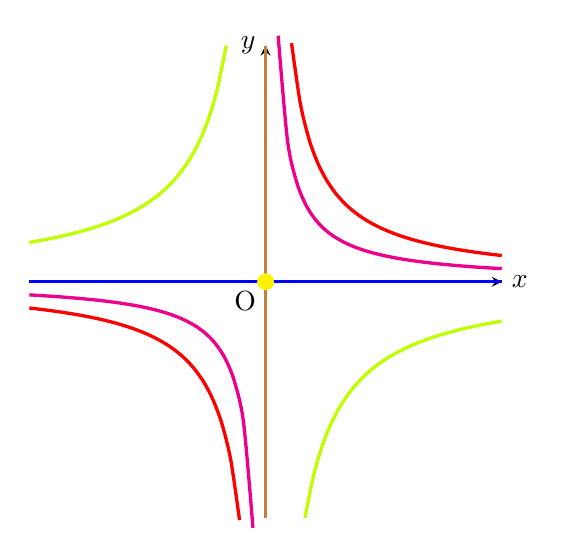
\begin{tikzpicture}[scale=1]

		\draw[->,>=stealth,semithick] (-3,0)--(3,0) node[right]{$x$}; %x軸
		\draw[->,>=stealth,semithick] (0,-3)--(0,3) node[left]{$y$}; %y軸
		\draw (0,0) node[below left]{O}; %原点
	
		\draw[domain=0.33:3,smooth,very thick,red] plot(\x,{1/\x});
		\draw[domain=-3:-0.33,smooth,very thick,red] plot(\x,{1/\x});
		\draw[domain=0.16:3,smooth,very thick,magenta] plot(\x,{1/(2*\x)});
		\draw[domain=-3:-0.16,smooth,very thick,magenta] plot(\x,{1/(2*\x)});
		\draw[domain=0.5:3,smooth,very thick,lime] plot(\x,{-3/(2*\x)});
		\draw[domain=-3:-0.5,smooth,very thick,lime] plot(\x,{-3/(2*\x)});
		\draw[blue,very thick,anchor=center](-3,0)--(3,0);
		\draw[brown,very thick,anchor=center](0,3)--(0,-3);
		\filldraw[yellow] (0,0) circle[radius=0.1];
	\end{tikzpicture}
\end{wrapfigure}
(1)点$(x,y)$の属す同値類を$[(x,y)]$と表す.
$x=y=0$なら$(x,y)$の同値類は$\{ (0,0)\}$である.
$x=0,y\neq0$のとき$(0,y)\sim(0,ty)\quad(t\in \mathbb{R}\setminus\{0\})$である.$y=0,x\neq0$のとき$(x,0)\sim (tx,0)\quad(t\in \mathbb{R}\setminus\{0\})$である.
$x\neq0\neq y$のとき$(x,y)\sim(x',y')\Leftrightarrow xy=x'y'$である.
したがって同値類は右のようになる.(異なる色は異なる同値類)

$x\neq 0 \neq y$なる$(x,y)$が含まれる同値類は$g(x,y)=xy$の逆像$g^{-1}(xy)$であるから閉集合.また$\{(0,0)\}$も閉集合である.
$[(0,y\neq0)]$は$(0,0)$が集積点であるが同値類に含まれないから閉集合ではない.同様に
$[(0\neq x,0)]$も閉集合ではない.

(2)$(0,0)$を含む$R^2$の開集合$\pi^{-1}(U)$に対してある$\varepsilon_U>0$が存在して
$B((0,0),\varepsilon_U)\subset \pi^{-1}(U)$となる.したがって$(x,0)\in \pi^{-1}(U)\quad(x\neq 0)$である.すなわち$[(0\neq x,0)]\in U$である.したがって$[(0\neq x,0)]$と$[(0,0)]$を分離する開集合は存在しないからハウスドルフでない.

(3)$i\le j$のとき同値類$[(1,1)]$上で$x^iy^j=y^{j-i}$となるから定数となるには$i=j$が必要.逆に$f(x,y)=\sum a_i (xy)^i$とするとこれは全ての同値類の上で定数である.

(4)$D=[(x,y)]\quad(x\neq 0\neq y)$のとき,$D\neq D'=[(x',y')]$に対して$xy\neq x'y'$である.したがって$h(x,y)=xy \in E$に対して$h(D)\neq h(D')$となる.
したがって$(*)$を満たす$D,D'$は共に$[(0,0)],[(0,1)],[(1,0)]$の何れか.
$f(x,y)=\sum a_i (xy)^i$について$f([(0,0)])=a_0,f([(0,1)])=a_0,f([(1,0)])=a_0$であるから求める対は$([(0,0)],[(0,1)]),([(0,0)],[(1,0)]),([(0,1)],[(1,0)])$及びこれらの順序を入れ替えたものである.

\fbox{3}
$A=\begin{pmatrix}
	1 & -1\\
	-1 & 1
	\end{pmatrix}$であるから$Ax+b=\begin{pmatrix}
		-x+y+b\\
		x-y+c
		\end{pmatrix}$である.よって$\langle Ax+b,x\rangle=-(x-y)^2+bx+cy$である.

$x+y=s,x-y=t$と変数変換すると$\langle Ax+b,x\rangle=-t^2+b\frac{s+t}{2}+c\frac{s-t}{2}$で,ヤコビアンは$-1/2$である.よって
\begin{align}
	I&=\int_{-\infty}^\infty \int_0^\infty \exp(-t^2+b\frac{s+t}{2}+c\frac{s-t}{2})\frac{1}{2}ds dt\\
	&= \frac{1}{2}\int_{-\infty}^\infty \exp(-(t-\frac{b-c}{4})^2+(\frac{b-c}{4})^2)dt \int_0^\infty \exp(\frac{b+c}{2}s)ds
\end{align}
である.$\int_{-\infty}^\infty \exp(-(t-\frac{b-c}{4})^2+(\frac{b-c}{4})^2)dt$は有限である.また$b+c<0$なら$\int_0^\infty \exp(\frac{b+c}{2}s)ds$も有限であり,$b+c\ge 0$なら発散する.

\fbox{4}
$f(z)$の$0$におけるローラン級数は$0$が極であることから正の整数$k$を用いて$\sum_{n=-k}^\infty a_n z^n$とかける.$z^kf(z)$は$|z|<2$で正則であり$\lim_{z\to 0} z^kf(z)=a_{-k}\neq 0$である.したがってある$\delta>0$が存在して$|z|<\delta$で
$|z^kf(z)|> |a_{-k}|/2$である.
したがって
\begin{align}
	 \iint_{\varepsilon<|z|<\delta} \frac{|a_{-k}|}{2|z|^k}dxdy&\le \iint_{\varepsilon<|z|<\delta} |f(z)|dxdy<\infty 
\end{align}である.$(x,y)=(r\cos \theta,r\sin \theta)$と極座標変換すると
$\int_\varepsilon^\delta \int_0^{2\pi} \frac{|a_{-k}|}{2r^k}rdrd\theta=|a_{-k}|\pi\int_{\varepsilon}^\delta |r^{1-k}|dr<\infty$である.$1-k\le-1$なら発散するから
$k<2$である.よって$k=1$より一位の極.


\end{document}